% Layout extracted from Kupzyk report at ca1d062; retain a descriptive title.
\documentclass[11pt]{article}
\usepackage[letterpaper,margin=0.82in]{geometry}
\usepackage{booktabs,longtable,array,graphicx,amsmath,xcolor,hyperref,xurl}
\usepackage[authoryear,round]{natbib}
\hypersetup{colorlinks=true,urlcolor=blue,linkcolor=blue,citecolor=blue}
\renewcommand{\arraystretch}{1.25}
\setlength{\emergencystretch}{1em}
\setlength{\parskip}{5pt}\setlength{\parindent}{0pt}
% Use scalable fonts; inspect pdffonts output after building. Avoid adding T1
% fontenc without an installed scalable font family. Add title/date in manuscript.

\newcommand{\repo}[2]{\href{https://github.com/alectionary/vibe-math/blob/master/formalization/pesah-biased-cubic/#1}{\nolinkurl{#2}}}
\title{Biased-noise thresholds of cubic and rhombic codes:\\a whole-dissertation replication audit of Pesah (2021)}
\author{}
\date{30 October 2026}
\begin{document}
\maketitle
\begin{abstract}
The dissertation's principal pure-Z advantage remains only partly reconstructed. Pesah reports cubic BP--OSD thresholds of 21.7\% undeformed and greater than 36\% deformed; we obtain 21.908\% for the former, but cannot identify a reliable asymptotic threshold for the latter. Rhombic pure-Z values are 28.4\% and 6.5\% in the source versus 27.407\% and 6.490\% here, retaining the strong disadvantage of that deformation. The preserved cubic pure-X comparison is 2.9\%/7.4\% versus 2.388\%/7.570\%. These are limited reconstructions with unknown original Monte Carlo error and production settings. A consequential point-estimate reversal occurs for cubic Sweep--Match depolarizing noise: the source deformation contrast is $+0.300$ percentage points, ours $-0.134$; our matching engine differs from the historical one. A cross-code ranking also reverses at Z bias 100, but the responsible cubic fit is unstable and does not establish a new ranking. A further 112,000 fresh trials expose size-dependent crossings; bounded logistic scaling is rejected in both tested local windows. General binary Hadamard and restricted-kernel lemmas are now checked in Lean, with source-semantic limits stated. The whole-dissertation objective remains open: full lattice proofs and historical-production/frontend equivalence are not complete. This expanded partial milestone does not claim that all results have been reproduced.
\end{abstract}

\section{Headline results and scope}
\begin{center}\begin{tabular}{llrrrrrr}
\toprule Code/decoder & Noise & \multicolumn{2}{c}{Source (\%)} & \multicolumn{2}{c}{Ours (\%)} & \multicolumn{2}{c}{$D-U$ (pp)}\\
 & & U & D & U & D & Source & Ours\\\midrule
Cubic BP & X & 2.9 & 7.4 & 2.388 & 7.570 & +4.5 & +5.182\\
Cubic BP & Z & 21.7 & $>36$ & 21.908 & unresolved & $>14.3$ & unresolved\\
Cubic BP & Dep. & 4.3 & 4.2 & 4.223 & 4.117 & -0.1 & -0.106\\
Cubic Sweep & X & 2.9 & 7.1 & 3.031 & 6.816 & +4.2 & +3.785\\
Cubic Sweep & Z & 14.7 & 22.2 & 14.182 & 19.473 & +7.5 & +5.291\\
Cubic Sweep & Dep. & 4.4 & 4.7 & 4.894 & 4.759 & +0.3 & -0.134\\
Rhombic BP & X & 1.0 & 1.7 & 1.047 & 1.864 & +0.7 & +0.817\\
Rhombic BP & Z & 28.4 & 6.5 & 27.407 & 6.490 & -21.9 & -20.916\\
Rhombic BP & Dep. & 1.5 & 1.7 & 1.640 & 1.649 & +0.2 & +0.009\\
\bottomrule\end{tabular}
\end{center}
U and D denote undeformed and deformed codes. Positive $D-U$ favors deformation. These are fitted point estimates, not established rankings. The table covers every endpoint cell of Tables 3.1--3.2; the deformed cubic Z source is an unresolved lower-bound statement, not an exact 36\% measurement. Ours-minus-source deviations are a different quantity, reported later. Fits with optimizer or model diagnostics are retained as outputs, not promoted to reliable thresholds.

Arthur Pesah's \emph{Tailoring 3D topological codes and decoders to biased noise} is a University College London \emph{Master of Research dissertation}, submitted 1 September 2021 under Dan Browne, not a doctoral thesis \citep{pesah2021}. We read all 66 pages. The initial milestone selected only cubic pure-X BP--OSD. The present objective covers every substantive dissertation result: endpoint thresholds, finite-bias comparisons, total/point/loop curves, code constructions and analytical reductions, the OSD optimization and the graphical interface. The original pure-X paper, code and results remain preserved. Background exposition and explicitly proposed future experiments are identified separately in \repo{coverage.json}{coverage.json}; none is silently counted as a reproduced original experiment.

The scientific question is whether local Hadamard deformation improves noise tolerance without changing physical-qubit count. The answer depends on code and channel. Cubic pure-X improves in the reconstruction; rhombic pure-Z worsens strongly. The larger cubic pure-Z claim remains unresolved. Resource equality, finite stabilizer checks, or agreement in one channel cannot substitute for that missing performance result.

\section{Experimental reconstruction}
We run periodic sizes $L=4,6,8,10$, both deformation arms, perfect syndrome measurements and independent physical-qubit errors. Categorical I/X/Y/Z draws preserve the simultaneous X and Z components of Y. For bias $\eta$ along one Pauli axis, its probability is $p\eta/(\eta+1)$ and each other axis receives $p/[2(\eta+1)]$. Depolarizing noise is $\eta=1/2$; the pure channels are the limiting cases. Hadamard deformation swaps X and Z on the selected axis.

The primary decoder reconstructs the historical ten-iteration BP and order-zero OSD implementation in \citet{bn3d}; its algorithmic context is \citet{roffe2020}. The source does not identify production seeds, counts, iteration settings, package versions, tie handling or fitting windows. Current NumPy quicksort, the historical prior regularizer and independent PCG64/MT19937 trials are explicit supplied assumptions. Full decoder equivalence to the undisclosed source production run is not established.

An original C++ GF(2) elimination routine accelerates OSD while preserving reliability ordering, pivot selection and zero free variables. It matched the preserved Python routine in 196 correction cases through $L=10$. The generalized cubic decoder matched 480 historical dense-reference cases; the rhombic implementation matched 320, after an explicit global Pauli conversion. These checks share graphs, priors and the stated algorithm. They independently check arithmetic/correction implementations, not an entire independent scientific replication.

The rhombic convention is consequential: the thesis prose uses cube Z checks and triangle X checks; the available historical code globally interchanges them. We use the prose convention and verify the exact global-Hadamard mapping. A nearby figure caption also conflicts with the prose. Table 3.2 calls the lattice cubic although its surrounding section and values describe rhombic. Figure 3.6 labels the undeformed pure-Z endpoint 21.0 percent versus Table 3.1's 21.7 percent; Figure 3.9 labels deformed depolarizing 1.6 percent versus Table 3.2's 1.7 percent. We retain table values for endpoint targets and record the figure discrepancies, rather than silently selecting whichever agrees best. This choice explains our channel labeling but does not prove which code revision generated the published plots.

Historical Sweep code is executed externally with PyMatching 2.3.1. The original 0.2.4 build required a LEMON archive whose host denied access. We did not retrieve it through another route. The modern sparse-blossom implementation \citep{higgott2025} is a disclosed engine departure. Eighty finite matching checks agree with independent exhaustive pairing of up to six defects, using shared shortest-path distances and graphs; they do not prove historical tie equivalence. All nonzero residual syndromes count as failures: 2,696 of 19,200 Sweep trials retain a residual syndrome. These are retained decoder failures, not discarded trials; all BP production corrections satisfy their syndromes.

The pure-Z grid contains 8,800 fresh trials and took approximately 2,478 seconds. The 28 BP families contain 179,200 trials; three Sweep families contain 19,200. Three wider diagnostic grids add 38,400. A further 5,600 shared-error diagnostic trials compare ten versus 100 BP iterations and stable versus quicksort ties (16,800 decoder executions). The full source-vertex curve run contains 226,800 trials; these production and wider-grid runs total 472,400. Individual production processes are capped at 2 GiB address space and 2,400 CPU seconds, with bounded worker concurrency. These counts exclude the preserved 16,000-trial pure-X milestone and small validation/pilot runs. Exact measured times, seeds and completion flags reside with each output. All production files passed completion, row-cardinality and count-integrity checks. Across separately reported families, 406 generator/seed keys are reused; those families are not pooled as independent evidence. The six cross-code contrasts use disjoint simulation seeds. Bonferroni requires no cross-test independence.

\section{Numerical agreement and uncertainty}
The source fits a quadratic finite-size form $y=A+Bx+Cx^2$, $x=(p-p_{\rm th})L^{1/\nu}$, by unweighted least squares (equations 3.1--3.2; see \citealp{tuckett2020}). We retain the initial bounded fit and separately report an exploratory normalized-$x$ reparameterization with relaxed coefficient/exponent bounds. Fits drop individual probability endpoints and extreme sizes as diagnostics. The normalized fit is not silently substituted for the original estimator.

Each two-arm family has 400 conditional binomial bootstrap draws. Bounds, nonphysical predictions and grid extrapolation prevent robust inference in several families. The expanded source-comparison family has 82 quantities: 24 BP families times three quantities, three Sweep families times three, and the undeformed cubic Z threshold. The preserved pure-X three-comparison family stays separate. We save unadjusted and Bonferroni-adjusted conditional bands; normal bands based on bootstrap standard errors are approximations, explicitly withheld as inference when diagnostics fail. Six cross-code contrasts form a separate family. These adjustments neither supply missing source uncertainty nor control finite-size/model bias.

\begin{longtable}{llrrl}
\toprule Family & Arm & Ours $-$ source (pp) & Conditional band (pp) & Rounding\\\midrule\endhead
cubic dep. & U & -0.077 & [-0.66, +0.51] & close\\
cubic dep. & D & -0.083 & [-0.57, +0.40] & close\\
rhombic dep. & U & +0.140 & [-0.31, +0.59] & close\\
rhombic dep. & D & -0.051 & [-0.38, +0.28] & close\\
rhombic X & U & +0.047 & [-0.11, +0.20] & match\\
rhombic X & D & +0.164 & [-0.77, +1.10] & mismatch\\
rhombic Z & U & -0.993 & [-4.02, +2.03] & mismatch\\
rhombic Z & D & -0.010 & [-0.92, +0.90] & match\\
sweep X & U & +0.131 & [-0.75, +1.01] & close\\
sweep X & D & -0.284 & [-1.61, +1.04] & mismatch\\
sweep Z & U & -0.518 & [-1.63, +0.59] & mismatch\\
sweep Z & D & -2.727 & [-4.75, -0.70] & mismatch\\
sweep dep. & U & +0.494 & [-0.18, +1.17] & mismatch\\
sweep dep. & D & +0.059 & [-0.51, +0.62] & close\\
cubic Z & U & +0.208 & [-3.28, +3.70] & mismatch\\
\bottomrule\end{longtable}

The displayed bands concern ours-minus-source deviations, in percentage points. They exclude unknown source Monte Carlo error. Table rounding uses half-up 0.1 pp precision: a match has identical rounding, and close is one last-place unit. Rounding remains distinct from uncertainty overlap and limited reconstruction scope. Figure coordinates have a conservative 0.1 pp extraction allowance, not an asserted original precision or trial error. Difference contrasts accumulate both input allowances.

Undeformed cubic pure-Z has bootstrap percentile interval 20.884--24.996\%, with four boundary fits among 400 draws; deleting an extreme size moves its estimate to 20.745--23.082\%. The deformed curve saturates and its sector fits hit boundaries. A numerical polynomial output around 42\% is therefore not reported as a resolved threshold. The source itself describes the 36--50\% crossing as uncertain.

Rhombic pure-Z yields a signed deformation contrast $-20.916$ pp versus source $-21.9$ pp. Its bootstrap fits have no optimizer-bound hits in this grid, but configuration and finite-size limits remain. The small rhombic depolarizing fitted advantage, $+0.009$ pp versus source $+0.2$ pp, does not establish a meaningful ranking. Sweep depolarizing changes from source $+0.300$ pp to ours $-0.134$ pp; seven bootstrap fits hit bounds, and modern matching further limits the comparison.

\section{Finite bias and cross-code comparisons}
\begin{longtable}{llrrrrr}
\toprule Code/axis & $\eta$ & \multicolumn{2}{c}{Source (\%)} & \multicolumn{2}{c}{Ours (\%)} & $D-U$: source/ours (pp)\\
 & & U & D & U & D & \\\midrule\endhead
Cubic X & 1 & 3.52 & 4.12 & 3.70 & 4.15 & +0.60/+0.45\\
Cubic X & 3 & 3.33 & 4.70 & 3.11 & 4.73 & +1.37/+1.61\\
Cubic X & 10 & 3.04 & 5.68 & 2.96 & 5.61 & +2.64/+2.65\\
Cubic X & 30 & 2.86 & 6.75 & 2.97 & 6.27 & +3.89/+3.30\\
Cubic X & 100 & 2.89 & 6.81 & 2.93 & 6.94 & +3.92/+4.02\\
Cubic Z & 1 & 5.56 & 5.08 & 5.57 & 4.94 & -0.48/-0.63\\
Cubic Z & 3 & 12.12 & 7.25 & 11.66 & 8.50 & -4.86/-3.16\\
Cubic Z & 10 & 22.35 & 12.44 & 22.51 & 13.19 & -9.92/-9.31\\
Cubic Z & 30 & 21.74 & 16.00 & 21.53 & 19.71 & -5.74/-1.82\\
Cubic Z & 100 & 21.71 & 23.75 & 21.03 & 37.83 & +2.04/+16.80\\
Rhombic X & 1 & 1.27 & 1.44 & 1.45 & 1.64 & +0.17/+0.20\\
Rhombic X & 3 & 1.16 & 1.50 & 1.22 & 1.63 & +0.34/+0.41\\
Rhombic X & 10 & 1.09 & 1.47 & 1.21 & 1.70 & +0.37/+0.49\\
Rhombic X & 30 & 1.07 & 1.59 & 1.04 & 1.80 & +0.52/+0.76\\
Rhombic X & 100 & 1.00 & 1.63 & 1.67 & 1.87 & +0.63/+0.20\\
Rhombic Z & 1 & 2.09 & 1.80 & 2.15 & 1.84 & -0.29/-0.31\\
Rhombic Z & 3 & 4.00 & 2.47 & 4.59 & 2.59 & -1.53/-1.99\\
Rhombic Z & 10 & 11.14 & 3.90 & 11.95 & 3.86 & -7.25/-8.08\\
Rhombic Z & 30 & 28.94 & 5.11 & 28.52 & 5.53 & -23.82/-23.00\\
Rhombic Z & 100 & 28.00 & 6.00 & 29.93 & 5.67 & -22.00/-24.26\\
\bottomrule\end{longtable}

Figure-derived source values above retain two decimal places only for readability; their extraction allowance is 0.1 pp. These are all plotted finite-bias conditions, with both arms and all four lattice sizes. The source methods list $\eta=5$ but vector plot coordinates put the corresponding point at 3. We run both; only 3 is compared with that plotted coordinate. Separate eta-5 results remain an alternative-method reconstruction without an invented source target.

Three wider independent grids were chosen after unstable fits. They remain exploratory: cubic Z eta-5 undeformed gives 18.905\% but nonphysical/nonmonotone polynomial predictions; cubic Z eta-100 deformed reaches the 49.99\% optimization bound outside the sampled grid; rhombic X eta-100 undeformed gives 0.725\% with some negative fitted probabilities. None resolves the affected original estimate simply by adding shots over a broader range.

The source ranks undeformed rhombic highest at Z bias 30--100. Five of six reconstructed pairwise point contrasts retain that direction. At eta-100, undeformed rhombic minus deformed cubic is $-7.898$ pp, reversing the source point ordering. The cubic fit is not identified reliably, including in the wider-grid check; this is evidence that the ranking is not reproduced robustly, not evidence for a new asymptotic winner. No source ranking is statistically established without its uncertainty.


\section{Fresh diagnostics for unstable finite-size fits}
We froze new grids using previous size-crossing brackets, without source thresholds as inputs, and ran 112,000 fresh trials at all four sizes. The two local families use 1,000 trials per generator and condition; the broad sector study uses 500. The 144 generator/seed pairs do not overlap the earlier expanded trials. Largest-size pilots used 60 trials each and cost 3.170, 0.364 and 2.460 seconds; two-worker production took 722.614 seconds, with peak resident memory below 70 MiB per process. Every BP correction was syndrome-valid. All earlier primary and wider-grid results remain unchanged.

\begin{center}
\begin{tabular}{lrrr}
\toprule Family & Local quadratic (\%) & Logistic (\%) & Deviance/16 df\\\midrule
Cubic Z, $\eta=5$, U & 20.5414 & 20.5725 & 137.219\\
Rhombic X, $\eta=100$, U & 1.05866 & 1.08223 & 56.699\\
\bottomrule
\end{tabular}
\end{center}
These are diagnostic fitted outputs, not accepted thresholds. The quadratic curves are physical and monotone on these frozen grids, unlike the earlier broad fits, but that alone does not establish scaling. The independently fitted bounded model is
$\operatorname{logit}(P)=a+b[(p-t)/\operatorname{median}(p)](L/6)^{1/\nu}$.
Its approximate goodness-of-fit probabilities are $2.52\times10^{-21}$ and $1.86\times10^{-6}$: both reject this model. Its profile intervals therefore are not reliable threshold intervals. This test does not test the different quadratic model's adequacy. Omitting the smallest or largest size is preserved as sensitivity, not used to select a favorable result. There is no unique plotted eta-5 source value because of the methods/figure discrepancy.

For cubic eta-5, the $L=4/6$, $4/8$ and $4/10$ interpolated crossings are 23.0704\%, 21.7571\% and 20.3394\%; the remaining pairs fail the predeclared uniqueness/stability guard. Corresponding rhombic crossings are 1.16486\%, 1.12861\% and 1.07830\%, with the other pairs likewise failing. A 12-member Bonferroni bootstrap family covers finite-grid interpolation conditionally on a unique root; it is not asymptotic threshold coverage. Missing, multiple or oppositely oriented crossings are retained, not fitted away.

Deformed cubic Z at eta-100 illustrates separate sector changes. At $L=10$, total/point/loop failure is $0.494/0.494/0$ at $p=.20$, $0.521/0.513/0.018$ at $.28$, and $0.887/0.513/0.764$ at $.40$. Eleven of 72 adjacent-size/sector signed differences exclude zero under conservative simultaneous exact-binomial intervals. All comparisons remain in the archive. No single global threshold is forced onto these curves, and the descriptive separation is not a causal or asymptotic proof. Point and loop failures share trials. Separate scalar likelihood and raw-count aggregation checks reproduce the analysis; they share the observations and model definitions, not an independent physical simulation.

\section{Full curve and analytical coverage}
The four pure-channel/code combinations cover total, point and loop failure for both arms and every size. The source supplies 6,804 factual vector coordinates across 96 curves. The reconstruction samples their horizontally displayed probability vertices, snapping calibrated coordinates to the source's 0.005 grid within extraction tolerance. Below-axis source values are treated as bounds rather than exact zero observations. The final comparison uses a declared 6,804-member Bonferroni Clopper--Pearson family for our binomial counts plus a 0.005 vertical extraction allowance; source trial counts remain unknown. All 6,804 source-coordinate intervals overlap our simultaneous bands, with zero invalid BP corrections in these 226,800 trials. This is a low-resolution compatibility check: only 100 fresh trials per condition and a large multiplicity family produce wide bands. It is not numerical equivalence, a recovered source trial archive, or evidence that every plotted value was exactly reproduced. The source has 4,322 visible vertices; the remaining below-axis coordinates are treated conservatively as probability intervals [0,0.015].

\begin{figure}[p]\centering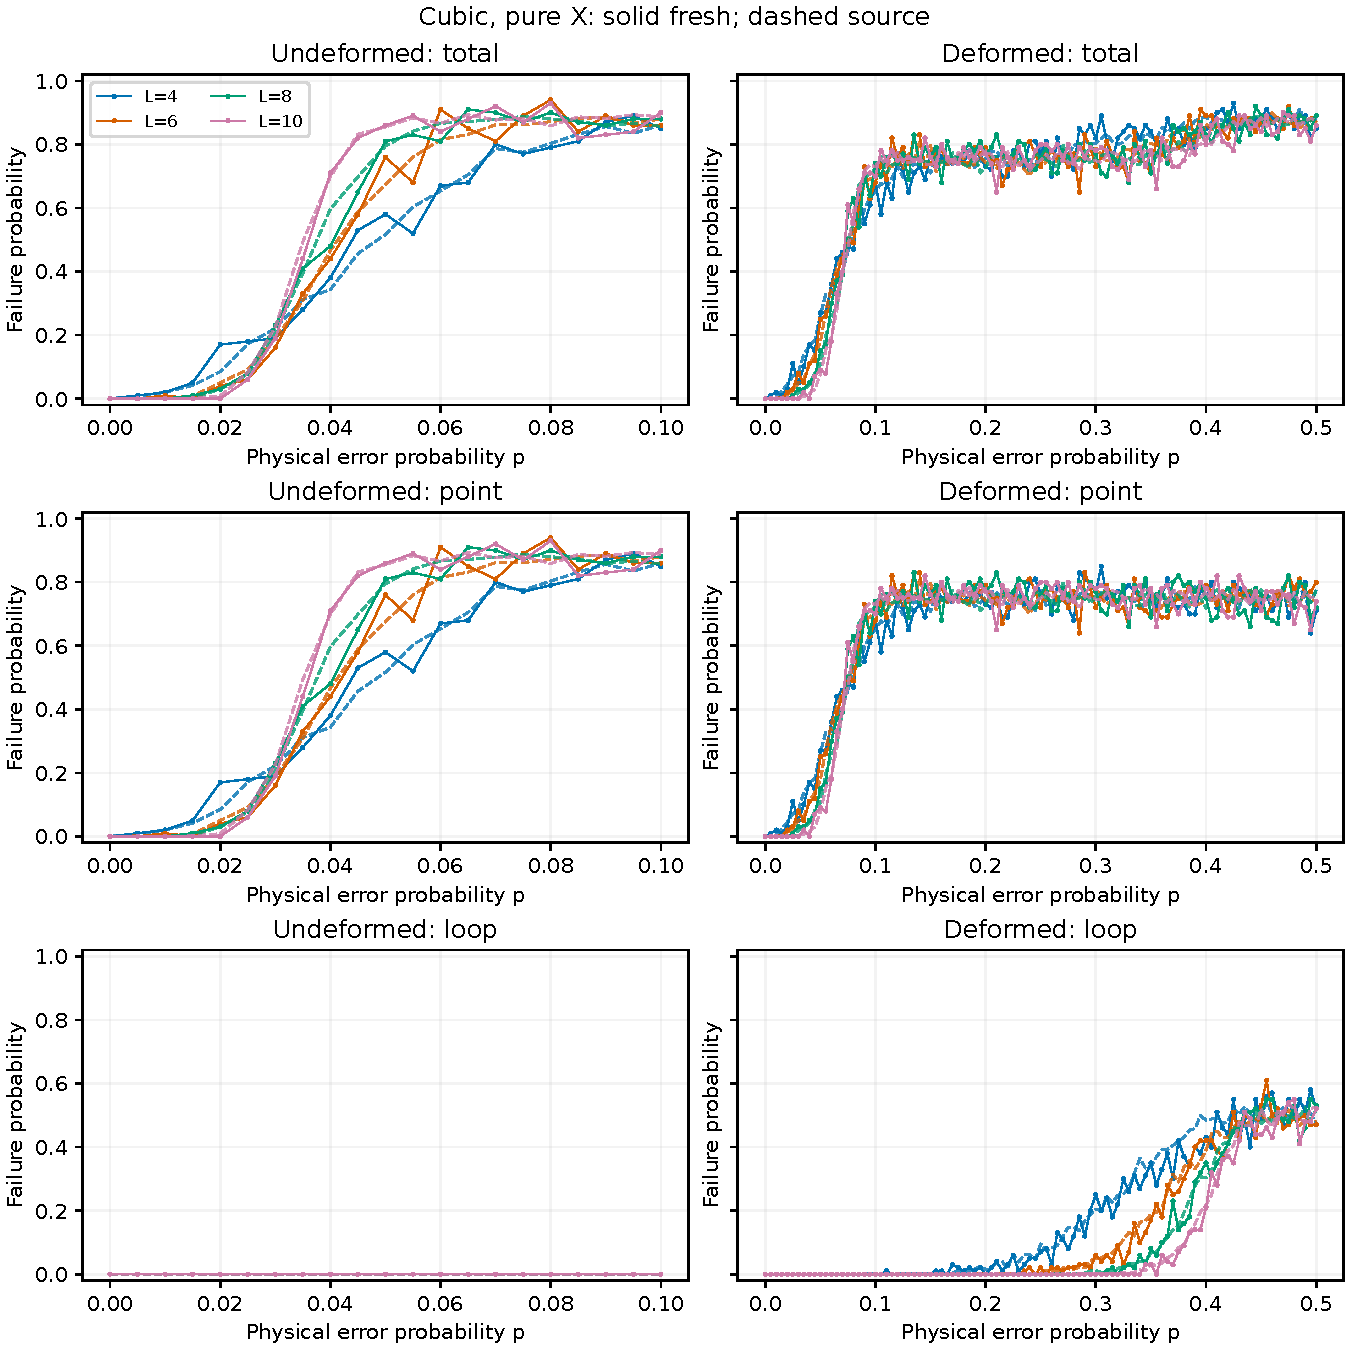
\includegraphics[width=.94\linewidth]{figures/expanded-cubic-X-curves.pdf}\caption{Cubic pure X: all sizes, arms and sectors. Solid lines are fresh trial frequencies; dashed lines are source vector coordinates. Connected lines guide the eye; no pointwise error bars imply simultaneous precision. Below-axis source coordinates are not exact observed zeros.}\end{figure}
\begin{figure}[p]\centering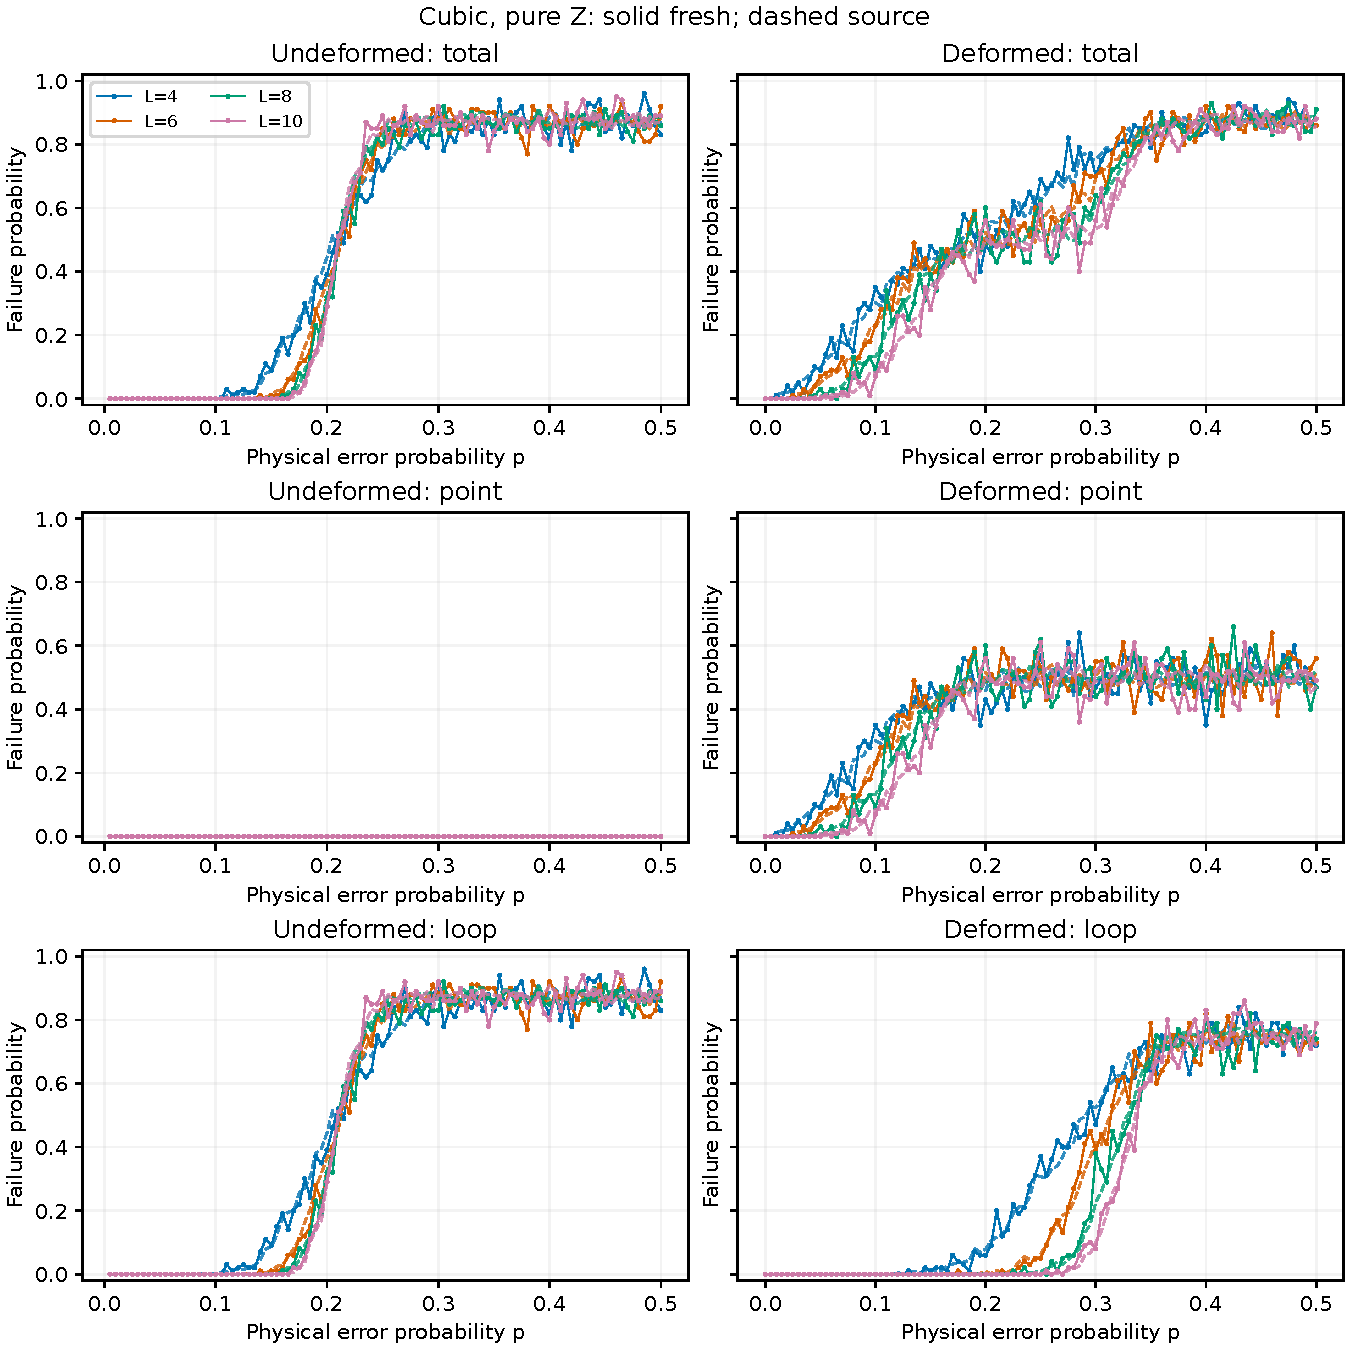
\includegraphics[width=.94\linewidth]{figures/expanded-cubic-Z-curves.pdf}\caption{Cubic pure Z: all sizes, arms and sectors. Solid lines are fresh trial frequencies; dashed lines are source vector coordinates. Connected lines guide the eye; no pointwise error bars imply simultaneous precision. Below-axis source coordinates are not exact observed zeros.}\end{figure}
\begin{figure}[p]\centering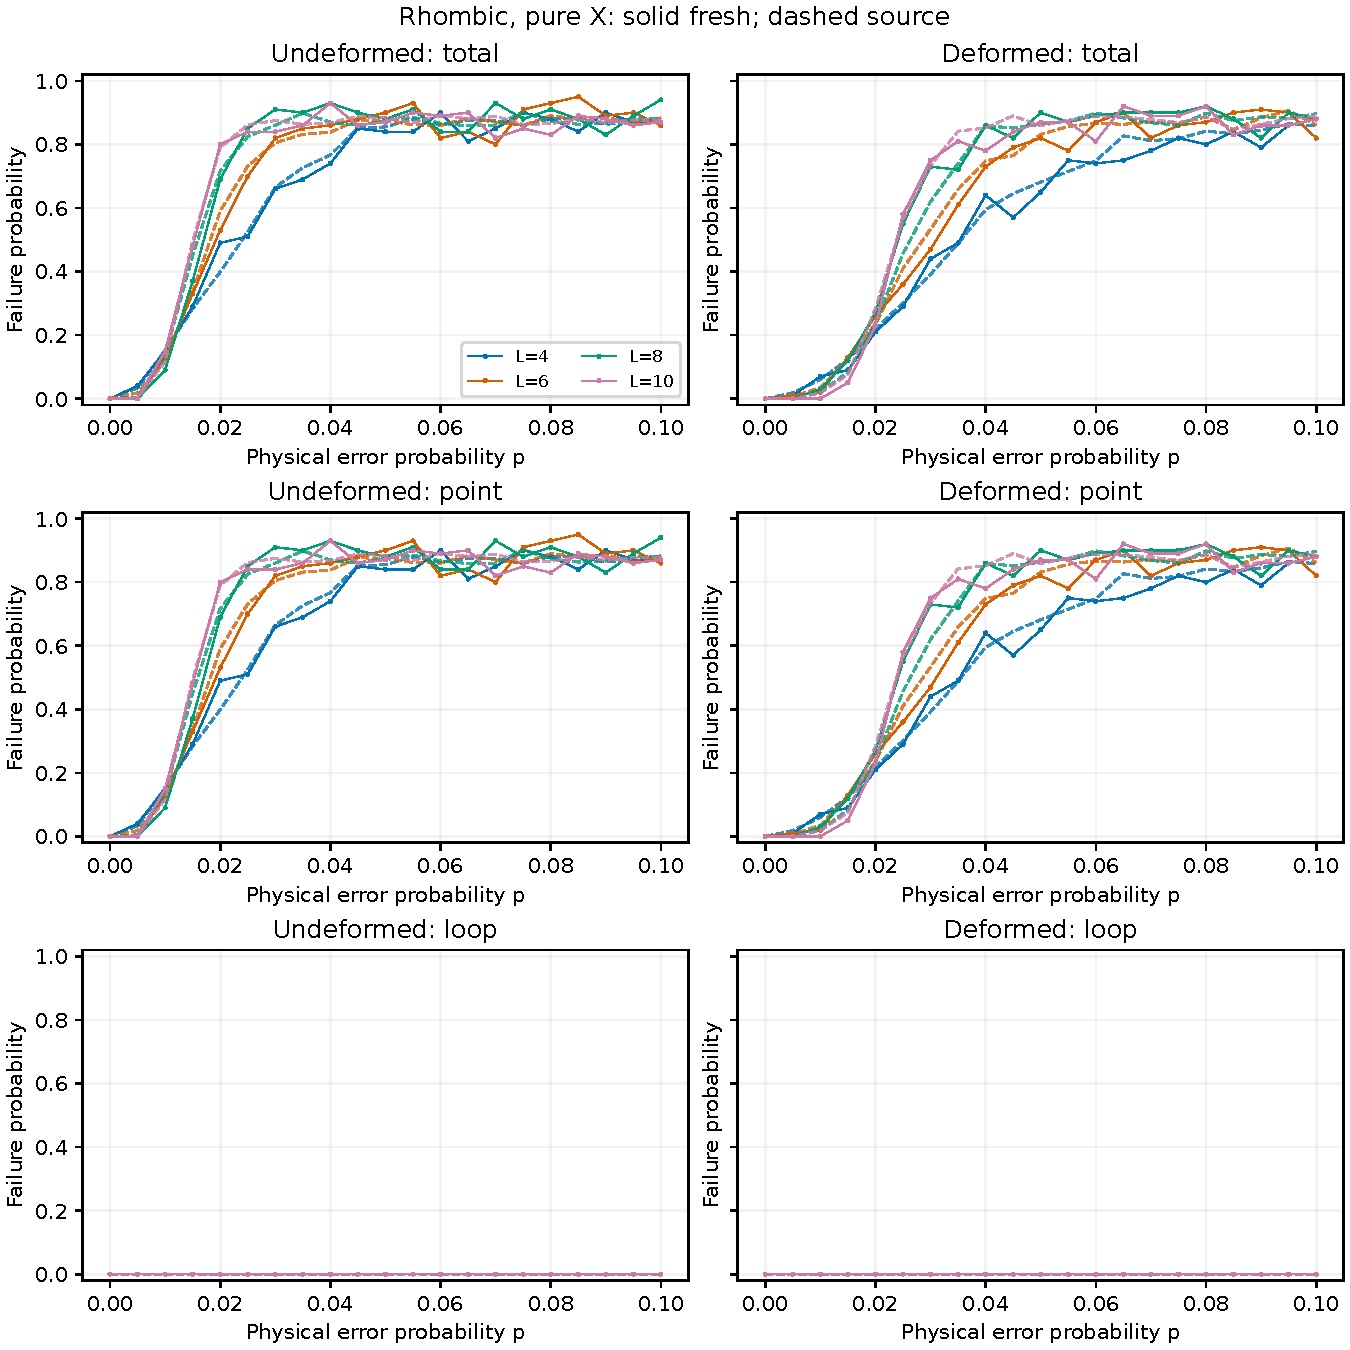
\includegraphics[width=.94\linewidth]{figures/expanded-rhombic-X-curves.pdf}\caption{Rhombic pure X: all sizes, arms and sectors. Solid lines are fresh trial frequencies; dashed lines are source vector coordinates. Connected lines guide the eye; no pointwise error bars imply simultaneous precision. Below-axis source coordinates are not exact observed zeros.}\end{figure}
\begin{figure}[p]\centering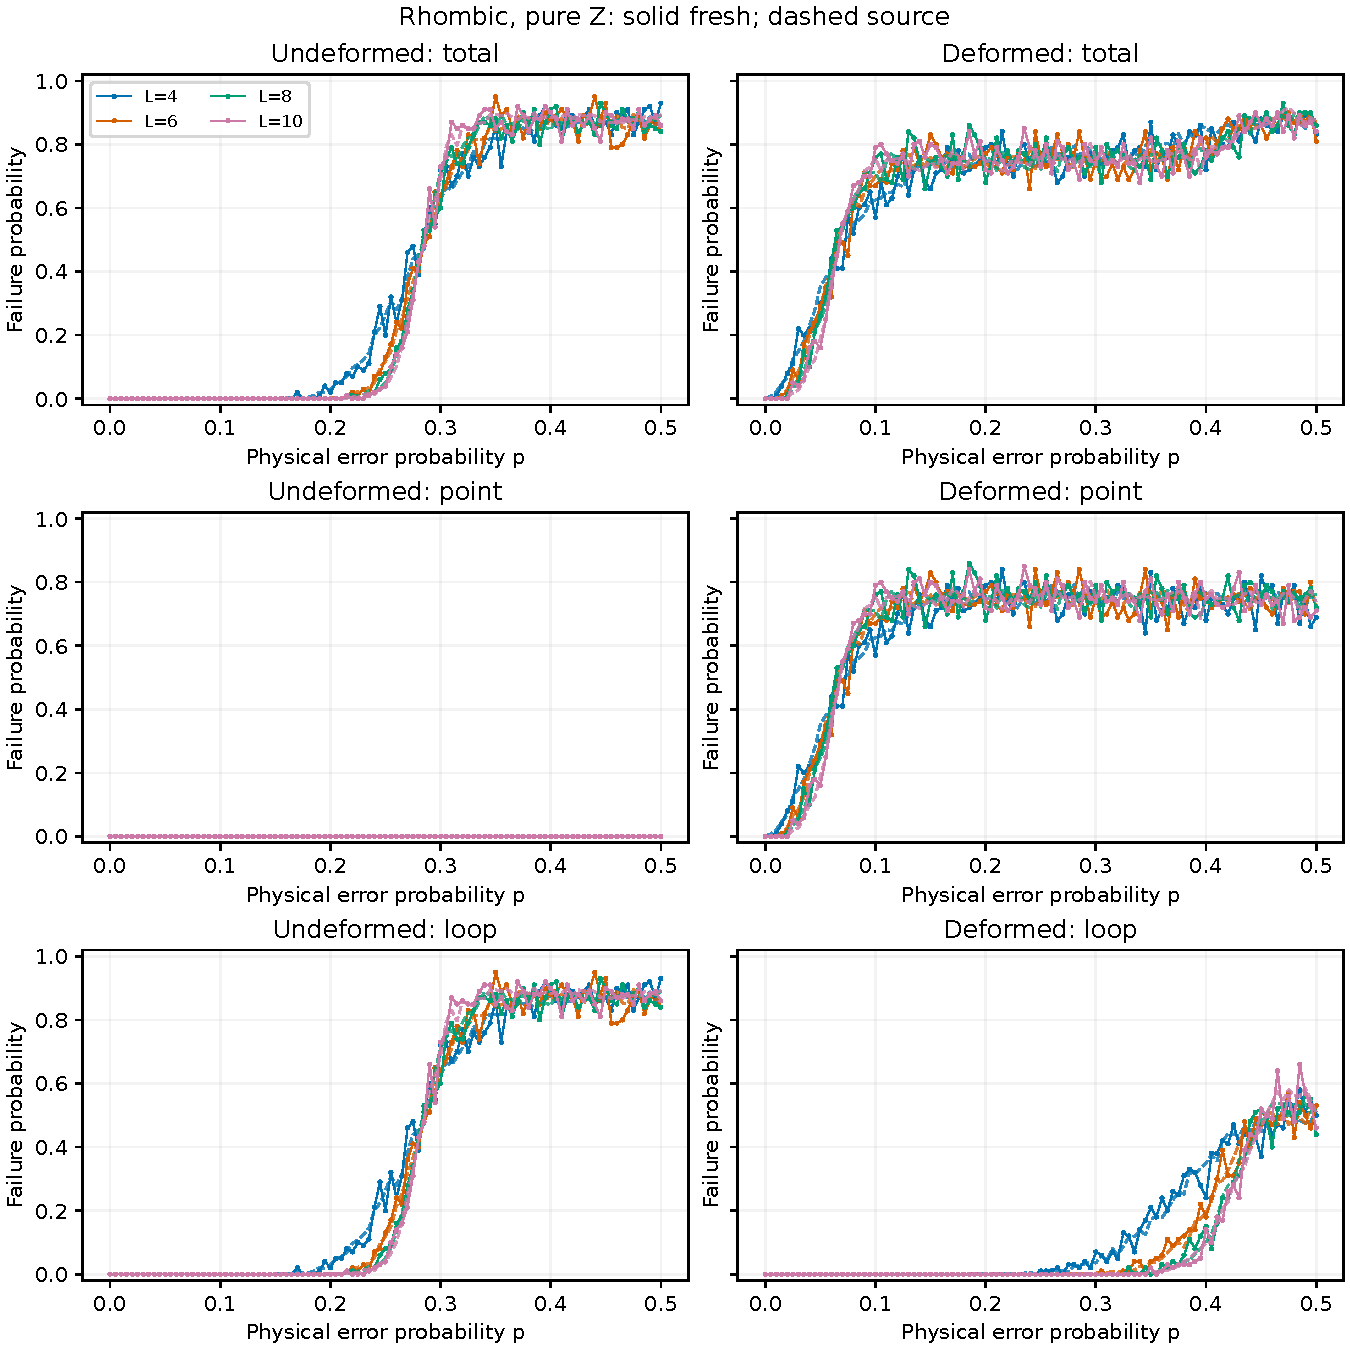
\includegraphics[width=.94\linewidth]{figures/expanded-rhombic-Z-curves.pdf}\caption{Rhombic pure Z: all sizes, arms and sectors. Solid lines are fresh trial frequencies; dashed lines are source vector coordinates. Connected lines guide the eye; no pointwise error bars imply simultaneous precision. Below-axis source coordinates are not exact observed zeros.}\end{figure}
\clearpage
Finite geometry checks establish commutation, three logical qubits, matched logical operators and restricted-axis nullities at $L=2,4,6,8,10$. Computational distance certificates verify matching lower and upper bounds at these sizes: cubic $d_X=L$, $d_Z=L^2$, and rhombic $d_X=L$, $d_Z=2L^2$ under our convention. The lower-bound check uses disjoint homologous representatives and exact row-space membership. These are finite computational certificates, not Lean proofs or an arbitrary-$L$ theorem.

For the ideal repetition-chain and plane reductions, a separate analytical audit evaluates finite binomial majority probabilities and parity composition, with explicit independent-component and random-tie assumptions. The 50\% ideal-sector limit is not the threshold of the actual BP--OSD decoder, nor does it establish the total-code threshold. The rhombic pure-X loop claim is checked through finite restricted-axis nullities. The follow-up now proves general binary Hadamard preservation and restricted difference-kernel formulas in Lean 4.22.0; the exact source bridges and remaining gaps are in Appendix B. These do not establish general lattice homology, distance formulas or ideal-decoder probability limits.

\section{Software contributions and attempted blockers}
The source claims a tenfold OSD speed improvement from reusing elimination rather than recomputing ranks. Our reconstructed repeated-rank baseline and reused-elimination implementation agree on 15 small cases and show speedups roughly 12--145 times. The original benchmark inputs, baseline implementation and hardware are absent; concurrent workload also affects our timings. This supports the mechanism, not an exact tenfold benchmark reproduction. The native optimization's separate speedup is not credited as a reproduction of that source claim.

On shared diagnostic errors, total failures are 1,375 at ten iterations, 1,476 at 100, and 1,353 with stable sorting, out of 5,600 each. These heterogeneous exploratory counts demonstrate setting sensitivity; they are not pooled threshold estimates. No invalid correction occurred in these checks.

The historical Flask backend passes 28 response checks: four code/size geometry checks and 24 zero-syndrome BP decoding requests. Browser loading of the original frontend encounters a denied external Three.js module host and produces no canvas. Frontend interaction/rendering remains blocked; no alternate CDN was used. Backend success is not full GUI reproduction. Claimed usefulness for visualization is qualitative and lacks a source evaluation protocol.

Chapter 4 proposes measurement/circuit noise, coprime dimensions, boundaries, higher-order OSD, a statistical-physics model and future resource comparisons. They are future work, not dissertation experiments that we failed to run. We do not invent circuit-level thresholds or Y-bias results merely because the setup mentions general Pauli channels.

\section{Availability, compliance and next steps}
The full source and external code remain outside this repository. Limited attributed evidence crops, vector factual coordinates and original reconstruction artifacts are governed by the repository's licensing notices. Source evidence: \repo{evidence/table3_1.png}{table3_1.png}, \repo{evidence/scaling_equations.png}{scaling_equations.png}, \repo{evidence/table3_2.png}{table3_2.png}, \repo{evidence/cubic_bias_figure.png}{cubic_bias_figure.png}, \repo{evidence/rhombic_bias_figure.png}{rhombic_bias_figure.png}, \repo{evidence/methods_grid.png}{methods_grid.png}, \repo{evidence/manifest.json}{manifest.json}, \repo{evidence/expansion-manifest.json}{expansion-manifest.json}. The following rows are copied from \repo{expanded-availability.md}{expanded-availability.md} and \repo{expanded-compliance.md}{expanded-compliance.md}. The original milestone ledgers remain separate.
\begin{longtable}{p{.23\linewidth}p{.70\linewidth}}
\toprule Item & Result and limit\\\midrule\endhead
Thesis and production archive & Complete 66-page author-hosted MRes source obtained at b4f401e0c12b44be4c69318e0015f70d8a3d3f98. All 47 returned author repositories and historical collaboration code searched; no pinned production trials/settings archive identified. Earlier search ledger retained; absence is not exhaustive.\\
Historical decoder source & PanQEC revision 686560e5d03c2e5d31f6c6260b03756af03a7e93 obtained externally. Dense BP and Sweep routines executed without vendoring. Exact dissertation production identity unknown.\\
Historical matching dependency & PyMatching0.2.4 could not be built: original setup fetched a LEMON archive from lemon.cs.elte.hu and received HTTP403. No alternate route or retry. PyMatching2.3.1 is a labeled reconstruction, not historical equivalence.\\
Graphical interface & Historical Flask backend tested. Original frontend requires cdn.skypack.dev/three@v0.130.1; CONNECT403 prevented module access and canvas rendering. No alternate CDN or host retry.\\
Unspecified research inputs & Original trial counts, seeds, BP settings, exact package pins, fitting windows and OSD benchmark workload/hardware were not found. Source uncertainty remains unknown. No author contact.\\
Permitted evidence & Eight attributed 600-dpi crops and factual vector coordinates retained with provenance; complete thesis and third-party source remain external. THIRD\_PARTY.md and LICENSING.md apply.\\
\bottomrule\end{longtable}

\begin{longtable}{p{.23\linewidth}p{.70\linewidth}}
\toprule Item & Result and limit\\\midrule\endhead
Objective and source status & Whole-dissertation objective, not selected-result completion. 87-item register includes numerical, analytical and software claims plus explicit background/future exclusions. Source is an MRes dissertation, not PhD; this selection departed from initial doctoral screening without asserting user-specific selection.\\
Skill and template & Replication skill and approved-preamble asset at revision 1e69e2c0e6fa2f42d0879d48936561df02659add; approved Kupzyk layout retained. Quantum BP/OSD and matching engines replace inapplicable SEM engines with recorded preflight. No reusable skill edits.\\
All numerical families & All source endpoint cells, finite plotted biases, eta5 method alternative and all pure-channel sector/arm/size curves attempted. Expanded production and wider grids: 472400 trials. Original pure-X milestone preserved. Unstable fits remain unresolved, not counted as successful thresholds.\\
Independent validation & 480 cubic and 320 rhombic historical dense correction matches; 196 native/Python OSD cases through L10; 80 modern matching/exhaustive-pairing cases. Shared inputs, graphs, priors and some software explicitly limit independence. Finite code/distance checks do not establish general theorems.\\
Resources and supplied defaults & Pure-Z pilot approximately 8.43/9.10 seconds per ten L10 trials; production 2478 seconds. Native optimization piloted before remaining families. Per-process 2400 CPU seconds and 2GiB address space, bounded workers and deterministic checkpoints. Ten BP iterations, order-zero OSD and current tie behavior are supplied assumptions.\\
Signed contrasts and precision & D minus U in pp favors deformation when positive. Separate ours-minus-source deviations. Sweep-depolarizing and eta100 cross-code point reversals disclosed with instability/engine limits. Printed table rounding, figure extraction, source uncertainty and reconstruction scope remain separate.\\
Uncertainty families & 82 expanded threshold/source quantities, six cross-code contrasts and 6804 curve-coordinate checks, each alpha0.05 Bonferroni; preserved pure-X family separate. Conditional bootstrap-normal bands flagged when fits fail diagnostics. Curve counts use exact binomial intervals. Missing source Monte Carlo and systematic errors are not repaired by multiplicity correction.\\
Sampling and failures & Distinct seeds within each run; 406 generator/seed keys overlap separately reported families, which are not pooled independently. Cross-code comparison seeds disjoint. All 2696 residual-syndrome Sweep trials count as failures; no invalid BP production correction.\\
Preservation and remaining work & Original pure-X code, analysis, bibliography and PDF preserved. Normalized and wider-grid diagnostics remain separate. General analytical proofs, exact historical runtime/production equivalence and frontend rendering are not complete. Coverage stays open.\\
Manuscript and delivery & Expanded main manuscript leads with headline numbers and limits, contains readable full-condition tables, source evidence and copied ledgers. Rendered PDF/scientific review and remote hash verification are separate acceptance gates; a successful build alone does not establish delivery.\\
Fresh follow-up & 112000 additional trials, zero invalid corrections, 722.614 seconds with two workers. Frozen source-independent grids; 12 crossing and 72 sector-contrast families. Logistic models rejected; no replacement threshold claim. Lean4.22 binary algebra and restricted kernels checked; full lattice/semantic/probability obligations remain open.\\
\bottomrule\end{longtable}


The whole-study register remains open for full lattice analytical proofs, semantic/probability bridges and investigation of unstable finite-size fits. The newly checked binary algebra does not close those obligations. Exact historical production reproduction additionally requires the missing job inputs, trial archive and environment; the matching and GUI source-access blockers are recorded precisely. No author contact was made.

\bibliographystyle{plainnat}
\bibliography{expanded-references}
\appendix
\section{Reproduction artifacts}
The preserved runnable pure-X revision is \href{https://github.com/alectionary/vibe-math/tree/47f111b60fbf668edc8fa6dfb4fb6a398d6da933/formalization/pesah-biased-cubic}{\nolinkurl{47f111b60fbf668edc8fa6dfb4fb6a398d6da933}}. It does not contain this expanded study. The immutable expanded runnable reproduction is \href{https://github.com/alectionary/vibe-math/blob/d1a437af56a24b4d35f6511f6be0d84d86a7157c/formalization/pesah-biased-cubic/expansion/README.md}{\nolinkurl{expansion/README.md}} at \nolinkurl{d1a437af56a24b4d35f6511f6be0d84d86a7157c}. New master navigation links await merge. The retained template is \repo{paper/approved-preamble.tex}{approved-preamble.tex}. See \repo{coverage.json}{coverage.json}, \repo{expansion/README.md}{expansion/README.md}, \repo{expansion/threshold-comparisons.json}{threshold-comparisons.json}, \repo{expansion/ranking-comparisons.json}{ranking-comparisons.json}, \repo{paper/expanded-manuscript.tex}{expanded-manuscript.tex} and \repo{paper/expanded-references.bib}{expanded-references.bib}. Main paper: \repo{paper/biased_noise_thresholds_of_cubic_and_rhombic_codes__replication_of_pesah_2021.pdf}{biased_noise_thresholds_of_cubic_and_rhombic_codes__replication_of_pesah_2021.pdf}.

\section{General algebra: proof-to-source correspondence}
The immutable follow-up runnable revision is
\href{https://github.com/alectionary/vibe-math/blob/8fac693b11097f44406ea699e2e502ce71461bb1/formalization/pesah-biased-cubic/followup/README.md}{\nolinkurl{followup/README.md}}
at \nolinkurl{8fac693b11097f44406ea699e2e502ce71461bb1}. It contains raw trials, frozen plans, analysis, validation and Lean source. Build with Lean 4.22.0 and Std only; \repo{followup/lean/build.sh}{build.sh} records the commands. All reported theorems compile without admitted proofs or added axioms; printed dependencies are only \texttt{propext} and \texttt{Quot.sound}. The following are standard algebraic reconstructions, not novelty claims.

\begin{longtable}{p{.20\linewidth}p{.35\linewidth}p{.35\linewidth}}
\toprule Source obligation & Exact checked statement & Remaining bridge\\\midrule\endhead
Hadamard, 2.3.3/3.2 & \nolinkurl{binary_parameters_preserved}: arbitrary finite qubits and swap mask preserve isotropic subgroup, basis-witness rank and minimum logical weight. & Binary Pauli modulo-phase semantics; Hilbert-space dimension/phase admissibility and actual lattice parameter formulas are separate.\\
Cubic chains, 3.2.1 & \nolinkurl{chain_kernel}: periodic first-axis differences vanish iff constant along each chain. & Actual incidence translation manually audited; cardinal/rank counting and majority-decoder probability limit not formalized.\\
Cubic planes, 3.4 & \nolinkurl{plane_kernel}: periodic y/z differences vanish iff constant on each yz-plane. & Same incidence/counting/probability limitations; no BP threshold implication.\\
Rhombic triangles, 3.5.2 & \nolinkurl{actual_two_corner_family_injective}: two restricted corner orientations expose every first-axis coordinate. & Formula-to-code translation manually audited; full even-periodic checkerboard geometry and Pauli convention remain separate.\\
\bottomrule\end{longtable}

A binary Pauli is a function $\{0,\ldots,n-1\}\to\mathrm F_2^2$. The deformation swaps its components on a chosen mask. The proof verifies involution, XOR linearity, support and full-qubit symplectic-product preservation. It then transports subgroup membership, normalizers, logical cosets, a generating independent list and exact minimum-weight witnesses. The definition of encoded qubits is the explicit basis-rank relation $n=r+k$, not an independently proved Hilbert-space dimension theorem. \nolinkurl{first_axis_parameters} instantiates $n=3L^3$ and the mask $i<L^3$, matching the Python first-third swap. No CSS sector-distance invariance is asserted after mixed deformation.

The periodic kernel proof uses induction around one coordinate: equality of adjacent bits implies constancy; applying it twice gives constant planes. In the cubic implementation, vertex restriction supplies neighboring first-axis edges (with a cyclic index shift), while the two face orientations supply y/z differences. The formal difference model allows positive lengths; the actual source lattice is used only at its stated admissible sizes, not a degenerate length-one implementation.

For rhombic triangles, the source reconstruction has one edge per axis and first-axis inward bit equal to base-X XOR vertex parity. Under first-axis-only error the other terms vanish. Orientations 0 and 2 supply base-X bits 0 and 1. Choosing base-X equal to vertex parity exposes the unshifted edge at every vertex, proving restricted-formula injectivity. This proof is stronger than the separate trivial coordinate-observation helper, but still does not formally extract the Python incidence matrix. The full code requires even periodic sizes; no odd-size physical result is claimed.

The remaining feasible obligations are arbitrary-size cubic/rhombic homology and distance lower bounds, source-incidence/counting bridges, ideal-majority probability limits, general BP/OSD correctness and unstable-fit adequacy. Historical production and GUI blockers remain distinct. A separate ownership-claim branch was denied by automatic approval review and was not retried; no reservation is asserted. That coordination limitation is recorded in \repo{followup/coordination.json}{coordination.json}.

\end{document}
